\chapter{Teoria dos Números}

\index{teoria dos números}

\key{Teoria dos números} é um ramo da matemática que estuda os números inteiros. A teoria dos números é um campo fascinante, pois muitas questões envolvendo números inteiros são muito difíceis de resolver, mesmo que pareçam simples à primeira vista.

Como exemplo, considere a seguinte equação:
\[x^3 + y^3 + z^3 = 33\]
É fácil encontrar três números reais $x$, $y$ e $z$ que satisfaçam a equação. Por exemplo, podemos escolher
\[
\begin{array}{lcl}
x = 3, \\
y = \sqrt[3]{3}, \\
z = \sqrt[3]{3}.\\
\end{array}
\]
No entanto, é um problema em aberto na teoria dos números se existem três \emph{números inteiros} $x$, $y$ e $z$ que satisfaçam a equação \cite{bec07}.

Neste capítulo, vamos nos concentrar em conceitos básicos e algoritmos em teoria dos números. Ao longo do capítulo, assumiremos que todos os números são inteiros, a menos que seja declarado de outra forma.

\section{Primos e Fatores}

\index{divisibilidade}
\index{fator}
\index{divisor}

Um número $a$ é chamado de \key{fator} ou \key{divisor} de um número $b$ se $a$ divide $b$. Se $a$ é um fator de $b$, escrevemos $a \mid b$, e caso contrário, escrevemos $a \nmid b$. Por exemplo, os fatores de 24 são 1, 2, 3, 4, 6, 8, 12 e 24.

\index{primo}
\index{fatoração em primos}

Um número $n>1$ é um \key{número primo} se seus únicos fatores positivos são 1 e $n$. Por exemplo, 7, 19 e 41 são primos, mas 35 não é primo, porque $5 \cdot 7 = 35$. Para cada número $n>1$, existe uma única \key{fatoração em primos}
\[ n = p_1^{\alpha_1} p_2^{\alpha_2} \cdots p_k^{\alpha_k},\]
onde $p_1,p_2,\ldots,p_k$ são primos distintos e $\alpha_1,\alpha_2,\ldots,\alpha_k$ são números positivos. Por exemplo, a fatoração em primos para 84 é
\[84 = 2^2 \cdot 3^1 \cdot 7^1.\]

A \key{quantidade de fatores} de um número $n$ é
\[\tau(n)=\prod_{i=1}^k (\alpha_i+1),\]
porque para cada primo $p_i$, existem $\alpha_i+1$ maneiras de escolher quantas vezes ele aparece no fator. Por exemplo, a quantidade de fatores de 84 é $\tau(84)=3 \cdot 2 \cdot 2 = 12$. Os fatores são 1, 2, 3, 4, 6, 7, 12, 14, 21, 28, 42 e 84.

A \key{soma dos fatores} de $n$ é
\[\sigma(n)=\prod_{i=1}^k (1+p_i+\ldots+p_i^{\alpha_i}) = \prod_{i=1}^k \frac{p_i^{a_i+1}-1}{p_i-1},\]
onde a última fórmula é baseada na fórmula da progressão geométrica. Por exemplo, a soma dos fatores de 84 é
\[\sigma(84)=\frac{2^3-1}{2-1} \cdot \frac{3^2-1}{3-1} \cdot \frac{7^2-1}{7-1} = 7 \cdot 4 \cdot 8 = 224.\]

O \key{produto dos fatores} de $n$ é
\[\mu(n)=n^{\tau(n)/2},\]
porque podemos formar $\tau(n)/2$ pares a partir dos fatores, cada um com produto $n$. Por exemplo, os fatores de 84 produzem os pares $1 \cdot 84$, $2 \cdot 42$, $3 \cdot 28$, etc., e o produto dos fatores é $\mu(84)=84^6=351298031616$.

\index{número perfeito}

Um número $n$ é chamado de \key{número perfeito} se $n=\sigma(n)-n$, ou seja, $n$ é igual à soma de seus fatores entre $1$ e $n-1$. Por exemplo, 28 é um número perfeito, porque $28=1+2+4+7+14$.

\subsubsection{Quantidade de Primos}

É fácil mostrar que existe um número infinito de primos. Se o número de primos fosse finito, poderíamos construir um conjunto $P=\{p_1,p_2,\ldots,p_n\}$ que conteria todos os primos. Por exemplo, $p_1=2$, $p_2=3$, $p_3=5$ e assim por diante. No entanto, usando $P$, poderíamos formar um novo primo
\[p_1 p_2 \cdots p_n+1\]
que é maior que todos os elementos em $P$. Isso é uma contradição, e a quantidade de primos tem que ser infinita.

\subsubsection{Densidade de Primos}

A densidade de primos significa com que frequência existem primos entre os números. Seja $\pi(n)$ a quantidade de primos entre $1$ e $n$. Por exemplo, $\pi(10)=4$, porque existem 4 primos entre $1$ e $10$: 2, 3, 5 e 7.

É possível mostrar que
\[\pi(n) \approx \frac{n}{\ln n},\]
o que significa que os primos são bastante frequentes. Por exemplo, a quantidade de primos entre $1$ e $10^6$ é $\pi(10^6)=78498$, e $10^6 / \ln 10^6 \approx 72382$.

\subsubsection{Conjecturas}

Existem muitas \emph{conjecturas} envolvendo primos. A maioria das pessoas pensa que as conjecturas são verdadeiras, mas ninguém foi capaz de prová-las. Por exemplo, as seguintes conjecturas são famosas:

\begin{itemize}
\index{Conjectura de Goldbach}
\item \key{Conjectura de Goldbach}:
Todo inteiro par $n>2$ pode ser representado como uma soma $n=a+b$ de forma que $a$ e $b$ sejam primos.
\index{primos gêmeos}
\item \key{Conjectura dos primos gêmeos}:
Existe um número infinito de pares da forma $\{p,p+2\}$, onde $p$ e $p+2$ são primos.
\index{Conjectura de Legendre}
\item \key{Conjectura de Legendre}:
Sempre existe um primo entre os números $n^2$ e $(n+1)^2$, onde $n$ é qualquer inteiro positivo.
\end{itemize}

\subsubsection{Algoritmos Básicos}

Se um número $n$ não é primo, ele pode ser representado como um produto $a \cdot b$, onde $a \le \sqrt n$ ou $b \le \sqrt n$, então certamente tem um fator entre $2$ e $\lfloor \sqrt n \rfloor$. Usando essa observação, podemos testar se um número é primo e encontrar a fatoração em primos de um número em tempo $O(\sqrt n)$.

A função a seguir, \texttt{primo}, verifica se um determinado número $n$ é primo. A função tenta dividir $n$ por todos os números entre $2$ e $\lfloor \sqrt n \rfloor$, e se nenhum deles dividir $n$, então $n$ é primo.

\begin{lstlisting}
bool primo(int n) {
    if (n < 2) return false;
    for (int x = 2; x*x <= n; x++) {
        if (n%x == 0) return false;
    }
    return true;
}
\end{lstlisting}

\noindent
A função a seguir, \texttt{fatores}, constrói um vetor que contém a fatoração em primos de $n$. A função divide $n$ por seus fatores primos e os adiciona ao vetor. O processo termina quando o número restante $n$ não tem fatores entre $2$ e $\lfloor \sqrt n \rfloor$. Se $n>1$, ele é primo e o último fator.

\begin{lstlisting}
vector<int> fatores(int n) {
    vector<int> f;
    for (int x = 2; x*x <= n; x++) {
        while (n%x == 0) {
            f.push_back(x);
            n /= x;
        }
    }
    if (n > 1) f.push_back(n);
    return f;
}
\end{lstlisting}

Observe que cada fator primo aparece no vetor tantas vezes quantas vezes divide o número. Por exemplo, $24=2^3 \cdot 3$, então o resultado da função é $[2,2,2,3]$.

\subsubsection{Crivo de Eratóstenes}

\index{crivo de Eratóstenes}

O \key{crivo de Eratóstenes}
%\footnote{Eratóstenes (c. 276 a.C. -- c. 194 a.C.) foi um matemático grego.}
é um algoritmo de pré-processamento que constrói um array usando o qual podemos verificar eficientemente se um determinado número entre $2 \ldots n$ é primo e, se não for, encontrar um fator primo do número.

O algoritmo constrói um array $\texttt{crivo}$ cujas posições $2,3,\ldots,n$ são usadas. O valor $\texttt{crivo}[k]=0$ significa que $k$ é primo, e o valor $\texttt{crivo}[k] \neq 0$ significa que $k$ não é primo e um de seus fatores primos é $\texttt{crivo}[k]$.

O algoritmo itera pelos números $2 \ldots n$ um por um. Sempre que um novo primo $x$ é encontrado, o algoritmo registra que os múltiplos de $x$ ($2x,3x,4x,\ldots$) não são primos, porque o número $x$ os divide.

Por exemplo, se $n=20$, o array é o seguinte:

\begin{center}
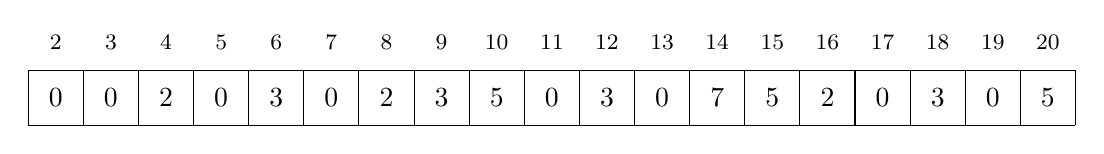
\begin{tikzpicture}[scale=0.7]
\draw (0,0) grid (19,1);

\node at (0.5,0.5) {$0$};
\node at (1.5,0.5) {$0$};
\node at (2.5,0.5) {$2$};
\node at (3.5,0.5) {$0$};
\node at (4.5,0.5) {$3$};
\node at (5.5,0.5) {$0$};
\node at (6.5,0.5) {$2$};
\node at (7.5,0.5) {$3$};
\node at (8.5,0.5) {$5$};
\node at (9.5,0.5) {$0$};
\node at (10.5,0.5) {$3$};
\node at (11.5,0.5) {$0$};
\node at (12.5,0.5) {$7$};
\node at (13.5,0.5) {$5$};
\node at (14.5,0.5) {$2$};
\node at (15.5,0.5) {$0$};
\node at (16.5,0.5) {$3$};
\node at (17.5,0.5) {$0$};
\node at (18.5,0.5) {$5$};

\footnotesize

\node at (0.5,1.5) {$2$};
\node at (1.5,1.5) {$3$};
\node at (2.5,1.5) {$4$};
\node at (3.5,1.5) {$5$};
\node at (4.5,1.5) {$6$};
\node at (5.5,1.5) {$7$};
\node at (6.5,1.5) {$8$};
\node at (7.5,1.5) {$9$};
\node at (8.5,1.5) {$10$};
\node at (9.5,1.5) {$11$};
\node at (10.5,1.5) {$12$};
\node at (11.5,1.5) {$13$};
\node at (12.5,1.5) {$14$};
\node at (13.5,1.5) {$15$};
\node at (14.5,1.5) {$16$};
\node at (15.5,1.5) {$17$};
\node at (16.5,1.5) {$18$};
\node at (17.5,1.5) {$19$};
\node at (18.5,1.5) {$20$};

\end{tikzpicture}
\end{center}

O código a seguir implementa o crivo de Eratóstenes. O código assume que cada elemento de $\texttt{crivo}$ é inicialmente zero.

\begin{lstlisting}
for (int x = 2; x <= n; x++) {
    if (crivo[x]) continue;
    for (int u = 2*x; u <= n; u += x) {
        crivo[u] = x;
    }
}
\end{lstlisting}

O loop interno do algoritmo é executado $n/x$ vezes para cada valor de $x$. Assim, um limite superior para o tempo de execução do algoritmo é a soma harmônica
\[\sum_{x=2}^n n/x = n/2 + n/3 + n/4 + \cdots + n/n = O(n \log n).\]

\index{soma harmônica}

Na verdade, o algoritmo é mais eficiente, porque o loop interno será executado apenas se o número $x$ for primo. Pode-se mostrar que o tempo de execução do algoritmo é apenas $O(n \log \log n)$, uma complexidade muito próxima de $O(n)$.

\subsubsection{Algoritmo de Euclides}

\index{máximo divisor comum}
\index{mínimo múltiplo comum}
\index{algoritmo de Euclides}

O \key{máximo divisor comum} de números $a$ e $b$, $\textrm{mdc}(a,b)$, é o maior número que divide $a$ e $b$, e o \key{mínimo múltiplo comum} de $a$ e $b$, $\textrm{mmc}(a,b)$, é o menor número que é divisível por $a$ e $b$. Por exemplo, $\textrm{mdc}(24,36)=12$ e $\textrm{mmc}(24,36)=72$.

O máximo divisor comum e o mínimo múltiplo comum estão conectados da seguinte forma:
\[\textrm{mmc}(a,b)=\frac{ab}{\textrm{mdc}(a,b)}\]

O \key{algoritmo de Euclides}\footnote{Euclides foi um matemático grego que viveu por volta de 300 a.C. Este é talvez o primeiro algoritmo conhecido na história.} fornece uma maneira eficiente de encontrar o máximo divisor comum de dois números. O algoritmo é baseado na seguinte fórmula:
\begin{equation*}
    \textrm{mdc}(a,b) = \begin{cases}
               a        & b = 0\\
               \textrm{mdc}(b,a \bmod b) & b \neq 0\\
           \end{cases}
\end{equation*}

Por exemplo,
\[\textrm{mdc}(24,36) = \textrm{mdc}(36,24)
= \textrm{mdc}(24,12) = \textrm{mdc}(12,0)=12.\]

O algoritmo pode ser implementado da seguinte forma:
\begin{lstlisting}
int mdc(int a, int b) {
    if (b == 0) return a;
    return mdc(b, a%b);
}
\end{lstlisting}

Pode-se mostrar que o algoritmo de Euclides funciona em tempo $O(\log n)$, onde $n=\min(a,b)$. O pior caso para o algoritmo é o caso em que $a$ e $b$ são números de Fibonacci consecutivos. Por exemplo,
\[\textrm{mdc}(13,8)=\textrm{mdc}(8,5)
=\textrm{mdc}(5,3)=\textrm{mdc}(3,2)=\textrm{mdc}(2,1)=\textrm{mdc}(1,0)=1.\]

\subsubsection{Função totiente de Euler}

\index{coprimo}
\index{função totiente de Euler}

Os números $a$ e $b$ são \key{coprimos} se $\textrm{mdc}(a,b)=1$. A \key{função totiente de Euler} $\varphi(n)$
%\footnote{Euler apresentou esta função em 1763.}
fornece a quantidade de números coprimos a $n$ entre $1$ e $n$. Por exemplo, $\varphi(12)=4$, porque 1, 5, 7 e 11 são coprimos a 12.

O valor de $\varphi(n)$ pode ser calculado a partir da fatoração em primos de $n$ usando a fórmula
\[ \varphi(n) = \prod_{i=1}^k p_i^{\alpha_i-1}(p_i-1). \]
Por exemplo, $\varphi(12)=2^1 \cdot (2-1) \cdot 3^0 \cdot (3-1)=4$. Observe que $\varphi(n)=n-1$ se $n$ é primo.

\section{Aritmética Modular}

\index{aritmética modular}

Na \key{aritmética modular}, o conjunto de números é limitado de forma que apenas os números $0,1,2,\ldots,m-1$ são usados, onde $m$ é uma constante. Cada número $x$ é representado pelo número $x \bmod m$: o resto após dividir $x$ por $m$. Por exemplo, se $m=17$, então $75$ é representado por $75 \bmod 17 = 7$.

Muitas vezes, podemos pegar os restos antes de fazer os cálculos. Em particular, as seguintes fórmulas são válidas:
\[
\begin{array}{rcl}
(x+y) \bmod m & = & (x \bmod m + y \bmod m) \bmod m \\
(x-y) \bmod m & = & (x \bmod m - y \bmod m) \bmod m \\
(x \cdot y) \bmod m & = & (x \bmod m \cdot y \bmod m) \bmod m \\
x^n \bmod m & = & (x \bmod m)^n \bmod m \\
\end{array}
\]

\subsubsection{Exponenciação Modular}

Muitas vezes, é necessário calcular eficientemente o valor de $x^n \bmod m$. Isso pode ser feito em tempo $O(\log n)$ usando a seguinte recursão:
\begin{equation*}
    x^n = \begin{cases}
               1        & n = 0\\
               x^{n/2} \cdot x^{n/2} & \text{$n$ é par}\\
               x^{n-1} \cdot x & \text{$n$ é ímpar}
           \end{cases}
\end{equation*}

É importante que, no caso de um $n$ par, o valor de $x^{n/2}$ seja calculado apenas uma vez. Isso garante que a complexidade de tempo do algoritmo seja $O(\log n)$, porque $n$ é sempre dividido pela metade quando é par.

A função a seguir calcula o valor de $x^n \bmod m$:

\begin{lstlisting}
int modpow(int x, int n, int m) {
    if (n == 0) return 1%m;
    long long u = modpow(x,n/2,m);
    u = (u*u)%m;
    if (n%2 == 1) u = (u*x)%m;
    return u;
}
\end{lstlisting}

\subsubsection{Teorema de Fermat e Teorema de Euler}

\index{Teorema de Fermat}
\index{Teorema de Euler}

O \key{Teorema de Fermat}
%\footnote{Fermat descobriu este teorema em 1640.}
afirma que
\[x^{m-1} \bmod m = 1\]
quando $m$ é primo e $x$ e $m$ são coprimos. Isso também resulta em
\[x^k \bmod m = x^{k \bmod (m-1)} \bmod m.\]
De forma mais geral, o \key{Teorema de Euler}
%\footnote{Euler publicou este teorema em 1763.}
afirma que
\[x^{\varphi(m)} \bmod m = 1\]
quando $x$ e $m$ são coprimos. O Teorema de Fermat segue do Teorema de Euler, porque se $m$ é primo, então $\varphi(m)=m-1$.

\subsubsection{Inverso Modular}

\index{inverso modular}

O inverso de $x$ módulo $m$ é um número $x^{-1}$ tal que
\[ x x^{-1} \bmod m = 1. \]
Por exemplo, se $x=6$ e $m=17$, então $x^{-1}=3$, porque $6\cdot3 \bmod 17=1$.

Usando inversos modulares, podemos dividir números módulo $m$, porque a divisão por $x$ corresponde à multiplicação por $x^{-1}$. Por exemplo, para avaliar o valor de $36/6 \bmod 17$, podemos usar a fórmula $2 \cdot 3 \bmod 17$, porque $36 \bmod 17 = 2$ e $6^{-1} \bmod 17 = 3$.

No entanto, um inverso modular nem sempre existe. Por exemplo, se $x=2$ e $m=4$, a equação
\[ x x^{-1} \bmod m = 1 \]
não pode ser resolvida, porque todos os múltiplos de 2 são pares e o resto nunca pode ser 1 quando $m=4$. Acontece que o valor de $x^{-1} \bmod m$ pode ser calculado exatamente quando $x$ e $m$ são coprimos.

Se um inverso modular existe, ele pode ser calculado usando a fórmula
\[
x^{-1} = x^{\varphi(m)-1}.
\]
Se $m$ é primo, a fórmula se torna
\[
x^{-1} = x^{m-2}.
\]
Por exemplo,
\[6^{-1} \bmod 17 =6^{17-2} \bmod 17 = 3.\]

Esta fórmula nos permite calcular eficientemente inversos modulares usando o algoritmo de exponenciação modular. A fórmula pode ser derivada usando o Teorema de Euler. Primeiro, o inverso modular deve satisfazer a seguinte equação:
\[
x x^{-1} \bmod m = 1.
\]
Por outro lado, de acordo com o Teorema de Euler,
\[
x^{\varphi(m)} \bmod m =  xx^{\varphi(m)-1} \bmod m = 1,
\]
então os números $x^{-1}$ e $x^{\varphi(m)-1}$ são iguais.

\subsubsection{Aritmética de Computador}

Na programação, inteiros sem sinal são representados módulo $2^k$, onde $k$ é o número de bits do tipo de dados. Uma consequência usual disso é que um número se repete se se tornar muito grande.

Por exemplo, em C++, números do tipo \texttt{unsigned int} são representados módulo $2^{32}$. O código a seguir declara uma variável \texttt{unsigned int} cujo valor é $123456789$. Depois disso, o valor será multiplicado por ele mesmo, e o resultado é $123456789^2 \bmod 2^{32} = 2537071545$.

\begin{lstlisting}
unsigned int x = 123456789;
cout << x*x << "\n"; // 2537071545
\end{lstlisting}

\section{Resolvendo Equações}

\subsubsection*{Equações Diofantinas}

\index{equação diofantina}

Uma \key{equação diofantina}
%\footnote{Diofanto de Alexandria foi um matemático grego que viveu no século III.}
é uma equação da forma
\[ ax + by = c, \]
onde $a$, $b$ e $c$ são constantes e os valores de $x$ e $y$ devem ser encontrados. Cada número na equação deve ser um inteiro. Por exemplo, uma solução para a equação $5x+2y=11$ é $x=3$ e $y=-2$.

\index{algoritmo de Euclides estendido}

Podemos resolver eficientemente uma equação diofantina usando o algoritmo de Euclides. Acontece que podemos estender o algoritmo de Euclides para que ele encontre números $x$ e $y$ que satisfaçam a seguinte equação:
\[
ax + by = \textrm{mdc}(a,b)
\]

Uma equação diofantina pode ser resolvida se $c$ for divisível por $\textrm{mdc}(a,b)$, caso contrário, não pode ser resolvida.

Como exemplo, vamos encontrar números $x$ e $y$ que satisfaçam a seguinte equação:
\[
39x + 15y = 12
\]
A equação pode ser resolvida porque $\textrm{mdc}(39,15)=3$ e $3 \mid 12$. Quando o algoritmo de Euclides calcula o máximo divisor comum de 39 e 15, ele produz a seguinte sequência de chamadas de função:
\[
\textrm{mdc}(39,15) = \textrm{mdc}(15,9)
= \textrm{mdc}(9,6) = \textrm{mdc}(6,3)
= \textrm{mdc}(3,0) = 3 \]
Isso corresponde às seguintes equações:
\[
\begin{array}{lcl}
39 - 2 \cdot 15 & = & 9 \\
15 - 1 \cdot 9 & = & 6 \\
9 - 1 \cdot 6 & = & 3 \\
\end{array}
\]
Usando essas equações, podemos derivar
\[
39 \cdot 2 + 15 \cdot (-5) = 3
\]
e multiplicando isso por 4, o resultado é
\[
39 \cdot 8 + 15 \cdot (-20) = 12,
\]
então uma solução para a equação é $x=8$ e $y=-20$.

Uma solução para uma equação diofantina não é única, porque podemos formar um número infinito de soluções se conhecermos uma solução. Se um par $(x,y)$ é uma solução, então todos os pares
\[(x+\frac{kb}{\textrm{mdc}(a,b)},y-\frac{ka}{\textrm{mdc}(a,b)})\]
também são soluções, onde $k$ é qualquer inteiro.

\subsubsection{Teorema Chinês do Resto}

\index{Teorema Chinês do Resto}

O \key{Teorema Chinês do Resto} resolve um grupo de equações da forma
\[
\begin{array}{lcl}
x & = & a_1 \bmod m_1 \\
x & = & a_2 \bmod m_2 \\
\cdots \\
x & = & a_n \bmod m_n \\
\end{array}
\]
onde todos os pares de $m_1,m_2,\ldots,m_n$ são coprimos.

Seja $x^{-1}_m$ o inverso de $x$ módulo $m$, e
\[ X_k = \frac{m_1 m_2 \cdots m_n}{m_k}.\]
Usando esta notação, uma solução para as equações é
\[x = a_1 X_1 {X_1}^{-1}_{m_1} + a_2 X_2 {X_2}^{-1}_{m_2} + \cdots + a_n X_n {X_n}^{-1}_{m_n}.\]
Nesta solução, para cada $k=1,2,\ldots,n$,
\[a_k X_k {X_k}^{-1}_{m_k} \bmod m_k = a_k,\]
porque
\[X_k {X_k}^{-1}_{m_k} \bmod m_k = 1.\]
Como todos os outros termos na soma são divisíveis por $m_k$, eles não têm efeito sobre o resto, e $x \bmod m_k = a_k$.

Por exemplo, uma solução para
\[
\begin{array}{lcl}
x & = & 3 \bmod 5 \\
x & = & 4 \bmod 7 \\
x & = & 2 \bmod 3 \\
\end{array}
\]
é
\[ 3 \cdot 21 \cdot 1 + 4 \cdot 15 \cdot 1 + 2 \cdot 35 \cdot 2 = 263.\]

Depois de encontrar uma solução $x$, podemos criar um número infinito de outras soluções, porque todos os números da forma
\[x+m_1 m_2 \cdots m_n\]
são soluções.

\section{Outros Resultados}

\subsubsection{Teorema de Lagrange}

\index{Teorema de Lagrange}

O \key{Teorema de Lagrange}
%\footnote{J.-L. Lagrange (1736--1813) foi um matemático italiano.}
afirma que todo inteiro positivo pode ser representado como a soma de quatro quadrados, ou seja, $a^2+b^2+c^2+d^2$. Por exemplo, o número 123 pode ser representado como a soma $8^2+5^2+5^2+3^2$.

\subsubsection{Teorema de Zeckendorf}

\index{Teorema de Zeckendorf}
\index{número de Fibonacci}

O \key{Teorema de Zeckendorf}
%\footnote{E. Zeckendorf publicou o teorema em 1972 \cite{zec72}; no entanto, este não foi um resultado novo.}
afirma que todo inteiro positivo tem uma representação única como uma soma de números de Fibonacci, de modo que não haja dois números iguais ou números de Fibonacci consecutivos. Por exemplo, o número 74 pode ser representado como a soma $55+13+5+1$.

\subsubsection{Ternas Pitagóricas}

\index{terna pitagórica}
\index{fórmula de Euclides}

Uma \key{terna pitagórica} é uma tripla $(a,b,c)$ que satisfaz o Teorema de Pitágoras $a^2+b^2=c^2$, o que significa que existe um triângulo retângulo com lados de comprimento $a$, $b$ e $c$. Por exemplo, $(3,4,5)$ é uma terna pitagórica.

Se $(a,b,c)$ é uma terna pitagórica, todas as triplas da forma $(ka,kb,kc)$ também são ternas pitagóricas, onde $k>1$. Uma terna pitagórica é \emph{primitiva} se $a$, $b$ e $c$ são coprimos, e todas as ternas pitagóricas podem ser construídas a partir de ternas primitivas usando um multiplicador $k$.

A \key{fórmula de Euclides} pode ser usada para produzir todas as ternas pitagóricas primitivas. Cada tripla desse tipo tem a forma
\[(n^2-m^2,2nm,n^2+m^2),\]
onde $0<m<n$, $n$ e $m$ são coprimos e pelo menos um de $n$ e $m$ é par. Por exemplo, quando $m=1$ e $n=2$, a fórmula produz a menor terna pitagórica
\[(2^2-1^2,2\cdot2\cdot1,2^2+1^2)=(3,4,5).\]

\subsubsection{Teorema de Wilson}

\index{Teorema de Wilson}

O \key{Teorema de Wilson}
%\footnote{J. Wilson (1741--1793) foi um matemático inglês.}
afirma que um número $n$ é primo exatamente quando
\[(n-1)! \bmod n = n-1.\]
Por exemplo, o número 11 é primo, porque
\[10! \bmod 11 = 10,\]
e o número 12 não é primo, porque
\[11! \bmod 12 = 0 \neq 11.\]

Portanto, o Teorema de Wilson pode ser usado para descobrir se um número é primo. No entanto, na prática, o teorema não pode ser aplicado a grandes valores de $n$, porque é difícil calcular valores de $(n-1)!$ quando $n$ é grande.
